\documentclass[pdflatex,sn-mathphys-num]{sn-jnl}% Math and 
\usepackage{graphicx}%
\usepackage{multirow}%
\usepackage{amsmath,amssymb,amsfonts}%
\usepackage{amsthm}%
%\usepackage{mathrsfs}%
\usepackage[title]{appendix}%
\usepackage{xcolor}%
\usepackage{textcomp}%
\usepackage{manyfoot}%
\usepackage{booktabs}%
\usepackage{algorithm}%
\usepackage{algorithmicx}%
\usepackage{algpseudocode}%
\usepackage{listings}%
\usepackage{tikz}
\usetikzlibrary{shapes.geometric, arrows.meta, positioning}

\theoremstyle{thmstyleone}%
\newtheorem{theorem}{Theorem}
\newtheorem{proposition}[theorem]{Proposition}

\theoremstyle{thmstyletwo}%
\newtheorem{example}{Example}%
\newtheorem{remark}{Remark}%

\theoremstyle{thmstylethree}%
\newtheorem{definition}{Definition}%

\raggedbottom

\begin{document}

\title[Article Title]{Disentangling Algorithmic Bias from Archival Artifacts: A Controlled Audit of Vision-Language Model Valuation in Metropolitan Museum Archives}

\abstract{
Auditing artificial intelligence models for societal bias requires distinguishing direct model evaluation disparities from confounders embedded within archival metadata. In this study, we audit visual-text representation and valuation bias in Contrastive Language-Image Pre-training (CLIP) models using artwork metadata harvested from the Metropolitan Museum of Art Open Access archives. We establish a multi-tiered quantitative framework, evaluating a corpus of historical artworks ($N = 1,500$ total objects; $N = 743$ attributed named works: Male $n = 534$, Female $n = 209$; $n = 618$ anonymous/unattributed) via zero-shot CLIP softmax probability differential scores across three distinct prompt formulations. Unadjusted evaluations demonstrate that zero-shot logit differentials across evaluated prompt pairs exhibit high residual embedding variance without a statistically significant main gender effect under either OpenAI CLIP ($\mu_F = -0.0067, \sigma = 0.0344$ vs $\mu_M = -0.0035, \sigma = 0.0361$; $U = 59,307.00$, $p = 0.1829$, rank-biserial $r = -0.0628$) or OpenCLIP ($\mu_F = 0.0171, \sigma = 0.0835$ vs $\mu_M = 0.0237, \sigma = 0.0886$; $U = 59,867.00$, $p = 0.1224$, $r = -0.0728$). Two One-Sided Tests (TOST) confirm statistical equivalence across Cohen's $d \ge 0.25$ bounds ($p_{\text{TOST}} = 0.0042$ at $d=0.30$ for OpenAI CLIP; $p_{\text{TOST}} = 0.0024$ for OpenCLIP). Prompt-level sensitivity checks confirm consistent valuation stability across semantic descriptors (\textit{masterpiece}, \textit{quality}, and \textit{influence}). Multivariate Ordinary Least Squares (OLS) regression controlling for physical artwork medium, creation century, and image aspect ratio ($R^2 = 0.018$, $F(11, 731) = 0.9286$, $p = 0.512$ for OpenAI CLIP; $R^2 = 0.017$, $F(11, 731) = 0.9888$, $p = 0.455$ for OpenCLIP) demonstrates that framing aspect ratio ($B = -0.0064, p = 0.141$ in CLIP; $B = -0.0023, p = 0.516$ in OpenCLIP) and artist gender ($B = 0.0037, p = 0.202$ in CLIP; $B = 0.0065, p = 0.356$ in OpenCLIP) exhibit no statistically significant main effect post-adjustment. Crucially, we highlight that zero-shot global prompt differentials exhibit high residual variance ($R^2 < 2\%$), indicating that global prestige metrics operate near an embedding noise floor where macro-level evaluations fail to isolate systematic demographic bias. We emphasize two central conceptual caveats: (i) macro-level zero-shot score equivalence does not preclude localized micro-level visual feature biases (e.g., subject gaze or compositional framing), and (ii) excluding $41.2\%$ ($n=618$) unattributed holdings reflects an uneliminable institutional survival bias, as named creators represent an already-sanitized subset of historical acquisition filters. These findings demonstrate the necessity of rigorous multivariate confound control, equivalence testing, and archival provenance auditing to prevent misattributing metadata curation artifacts to demographic model bias.
}

\keywords{Vision-Language Models, Algorithmic Bias Audits, Museum Archives, Digital Humanities, Confound Control, Responsible AI}

\maketitle

\section{Introduction}
\label{sec:introduction}

\subsection{Background and Motivation}
Large-scale vision-language models (VLMs), such as Contrastive Language-Image Pre-training (CLIP) \cite{radford2021learning}, are increasingly deployed across digital humanities, automated collection cataloging, and computational art history \cite{fiorucci2020machine, garcia2020bias}. Because these models align visual features with text representations learned from uncurated web scrapes, concern has grown that they inherit and amplify historical socio-cultural biases \cite{birhane2021multimodal, wolfe2022evidence, bender2021stochastic}. In cultural heritage institutions, historical collections already reflect systemic representational imbalances, including severe gender and regional disparities in acquisition and archival documentation \cite{topaz2019diversity, meier2021gender, carlson2022museum, bailey2020gender, nochlin1971why, pollock1988vision}.

When auditing VLMs for representational bias, a critical methodological challenge arises: distinguishing direct algorithmic valuation bias from confounding variables embedded within archival metadata \cite{hall2023auditing, buolamwini2018gender, noorthuis2020bias}. Grounded in established Responsible AI governance frameworks \cite{dignum2019responsible, stahl2021responsible, jobin2019global} and critical studies of classification infrastructures \cite{bowker2000sorting, noble2018algorithms, pasquale2015black}, evaluating AI fairness in cultural archives requires controlled quantitative audit pipelines capable of isolating demographic main effects from structural collection artifacts. In critical archival studies, classification taxonomies are recognized not as neutral administrative tools, but as sociotechnical infrastructures that embed historical power relations, institutional boundaries, and gendered labor exclusions \cite{bowker2000sorting, noble2018algorithms}. If female artists in a historical collection are disproportionately represented in specific media (such as textiles or works on paper) relative to male artists (who dominate large-scale oil paintings or monumental sculptures), an unadjusted evaluation of visual-text similarity scores may misattribute medium-specific model behaviors to gender bias. Embedding multivariate confound control directly into Responsible AI audit architectures \cite{mitchell2019model, stahl2021responsible} ensures that institutional AI deployments do not misinterpret historical curation artifacts as active model evaluation bias.

Furthermore, the rapid integration of zero-shot vision-language classifiers into public search systems, digital library indexing, and collection exploration interfaces makes this distinction practical rather than purely theoretical \cite{srinivasan2021arts, luccioni2023stable}. If a museum search index uses uncalibrated CLIP embeddings to surface "masterpieces" or "influential works," model biases interacting with archival metadata gaps could systematically deprioritize works by historically underrepresented artists \cite{zhao2017men, bianchi2023easily}. Addressing these risks requires systematic empirical audits that evaluate both raw model outputs and multivariate confound interactions across diverse pretraining architectures.

\subsection{Research Questions and Core Contributions}
This study investigates how vision-language models evaluate historical artworks and whether observed score disparities reflect direct artist gender bias or underlying archival confounders. We address three central research questions:
\begin{enumerate}
    \item \textbf{RQ1:} Do CLIP visual-text similarity scores assign significantly lower aesthetic valuation to artworks created by female artists compared to male artists in public museum collections?
    \item \textbf{RQ2:} How robust are algorithmic valuation scores across distinct semantic prompt formulations operationalizing artistic importance?
    \item \textbf{RQ3:} When controlling for structural archival confounders such as artwork medium, historical creation era, and aspect ratio, does artist gender remain a statistically significant predictor of model evaluation?
\end{enumerate}

To answer these questions, we audit a complete corpus of historical artworks ($N = 1,500$ total records: $N = 743$ attributed works, Male $n = 534$, Female $n = 209$; $n = 618$ anonymous/unattributed) harvested from the Metropolitan Museum of Art Open Access API \cite{met_api_2023, garcia2020bias}. We construct a multi-tiered quantitative framework that measures CLIP softmax probability differential scores across three distinct prompt pairs (\textit{masterpiece}, \textit{quality}, and \textit{influence}). We apply non-parametric hypothesis testing (Mann-Whitney $U$), rank-biserial effect sizes ($r$), bootstrapped 95\% confidence intervals, and multivariate Ordinary Least Squares (OLS) regression with HC3 heteroskedasticity-robust standard errors across two model pretraining regimes: OpenAI CLIP (ViT-B/32, trained on curated WIT) and OpenCLIP (ViT-B/32, trained on uncurated LAION-2B) \cite{cherti2023reproducible, schuhmann2022laion}.

Our primary empirical contributions include:
\begin{itemize}
    \item Unadjusted evaluations across the complete $N=743$ attributed corpus demonstrate high score convergence without a statistically significant composite gender valuation gap between female and male artists under OpenAI CLIP ($\mu_F = -0.0067$ vs $\mu_M = -0.0035, U = 59,307.00, p = 0.1829, r = -0.0628$) or OpenCLIP ($\mu_F = 0.0171$ vs $\mu_M = 0.0237, U = 59,867.00, p = 0.1224, r = -0.0728$).
    \item Two One-Sided Tests (TOST) establish formal statistical equivalence between male and female artwork score distributions across Cohen's $d \ge 0.25$ equivalence bounds ($p_{\text{TOST}} = 0.0042$ at $d=0.30$ for OpenAI CLIP; $p_{\text{TOST}} = 0.0024$ for OpenCLIP), supported by sensitivity checks across bounds $d \in [0.15, 0.40]$.
    \item Prompt sensitivity checks demonstrate robust consistency across all semantic descriptors (\textit{masterpiece}, \textit{quality}, and \textit{influence}), with no statistically significant individual prompt shifts surviving baseline controls or Bonferroni adjustment.
    \item Multivariate OLS regression controlling for medium, creation century, and framing aspect ratio ($R^2 = 0.018, F(11, 731) = 0.9286, p = 0.512$ for CLIP; $R^2 = 0.017, F(11, 731) = 0.9888, p = 0.455$ for OpenCLIP) confirms that artist gender ($B = 0.0037, p = 0.202$ for OpenAI CLIP; $B = 0.0065, p = 0.356$ for OpenCLIP) and aspect ratio ($B = -0.0064, p = 0.141$ for CLIP; $B = -0.0023, p = 0.516$ for OpenCLIP) exhibit non-significant conditional effects. Low total $R^2$ ($<2\%$) reflects high residual embedding variance, demonstrating that zero-shot global prompt metrics operate near a noise floor where macro-level evaluations are dominated by embedding variance rather than systematic demographic bias.
    \item We contextualize these findings within institutional archival boundaries, emphasizing the \textit{Archival Survival Bias Paradox}: filtering out $41.2\%$ ($n=618$) unattributed objects introduces dataset selection bias by auditing only named creators who already survived institutional gatekeeping while omitting the archival strata where female domestic craft labor was historically erased.
\end{itemize}

\subsection{Scope and Target Framework}
This work aligns directly with Responsible AI governance frameworks in archival and digital humanities practice \cite{dignum2019responsible, stahl2021responsible, mitchell2019model, jobin2019global}. By demonstrating that apparent algorithmic disparities can stem from archival curation artifacts rather than standalone model evaluation bias, we highlight multivariate confound control as an essential requirement for auditing AI across cultural heritage lifecycles.

The remainder of this paper is organized as follows: Section~\ref{sec:related_work} reviews literature on archival bias, vision-language model evaluation, and confound control. Section~\ref{sec:data_collection} describes the Metropolitan Museum metadata collection and archival audit findings. Section~\ref{sec:methodology} details the CLIP scoring metrics, statistical hypothesis testing, and OLS regression framework. Section~\ref{sec:results} presents empirical results. Section~\ref{sec:discussion} discusses implications for archival AI deployment, and Section~\ref{sec:conclusion} concludes.


\section{Related Work}
\label{sec:related_work}

\subsection{Representational Disparities in Cultural Heritage Archives}
Cultural heritage archives and museum collections reflect historical patterns of institutional acquisition, patronage, and societal exclusion \cite{carlson2022museum, meier2021gender, bailey2020gender}. Quantitative surveys of major Western art archives demonstrate substantial representational imbalances across artist gender and geographic origin \cite{topaz2019diversity}. Systemic analysis of holdings across prominent U.S. art museums indicates that over 85\% of cataloged artists are male and predominantly Euro-American \cite{topaz2019diversity}. These structural imbalances stem from historical barriers to institutional access, restricted entry to royal academies, patron preferences, and archival documentation practices where metadata fields for marginalized groups remain sparse or unindexed \cite{garcia2020bias, noorthuis2020bias}.

Digitization of museum collections via public Application Programming Interfaces (APIs)—such as those provided by the Metropolitan Museum of Art and Europeana—has enabled large-scale computational art history and digital humanities research \cite{fiorucci2020machine, met_api_2023}. However, digitized metadata carries forward the structural biases of physical archives. When computational pipelines process museum APIs without accounting for historical metadata gaps, representational asymmetries risk being interpreted as inherent features of cultural production rather than artifacts of institutional curation \cite{dignum2019responsible}.

In critical archival studies, classification systems are recognized not as neutral administrative tools, but as sociotechnical infrastructures that embed historical power relations and institutional boundaries \cite{bowker2000sorting, noble2018algorithms, caswell2017archival}. When vision-language models process digitized museum metadata, they do not merely extract visual features; they re-encode historical taxonomic classifications that historically prioritized canonical Western fine art (such as oil paintings and monumental sculpture) over decorative, domestic, and textile media \cite{bailey2020gender, bowker2000sorting}. Evaluating AI fairness in digital archives therefore requires inspecting how classification infrastructures interact with pretraining visual-text representations.

\subsection{Algorithmic Valuation in Vision-Language Models}
Contrastive Language-Image Pre-training (CLIP) \cite{radford2021learning} and related multimodal vision-language models (VLMs) align visual and text representations by joint optimization over web-scraped image-text pairs \cite{he2016deep, dosovitskiy2020image}. While CLIP achieves strong zero-shot classification performance, pretraining datasets ingest pervasive social stereotypes, demographic biases, and valuation skews \cite{birhane2021multimodal, wolfe2022evidence, bender2021stochastic, steed2021image}.

In visual domain audits, VLMs exhibit bias when evaluating human traits, professional roles, and aesthetic concepts \cite{hall2023auditing, wang2022revisiting, luccioni2023stable}. Specifically, when prompted with value-laden terms (such as \textit{masterpiece}, \textit{high quality}, or \textit{influential}), VLMs compute cosine similarities that reflect learned cultural associations between visual features and subjective value judgments \cite{garcia2020bias, bianchi2023easily}. When applied to cultural artifacts, these models risk operationalizing normative value judgments that privilege traditional Western fine art over decorative arts, textiles, or non-canonical media, indirectly penalizing artist demographics historically associated with those media \cite{wolfe2022evidence, zhao2017men}.

\subsection{Confound Control in Multimodal AI Audits}
A growing body of algorithmic fairness literature highlights the risk of confounding in observational AI audits \cite{buolamwini2018gender, mitchell2019model, bolukbasi2016man}. Observational evaluations that compare raw model score outputs across demographic groups without controlling for correlated structural covariates often report spurious bias metrics \cite{hall2023auditing}. Early audits in facial analysis demonstrated that classification disparities were driven by lighting and skin tone interactions rather than standalone gender predictors \cite{buolamwini2018gender}.

In digital heritage, observational evaluations of model behavior face severe confounding from physical artwork attributes, including artistic medium, physical dimensions, historical era, and digitized image resolution \cite{fiorucci2020machine, meier2021gender}. Medium distributions in historical collections are non-randomly correlated with artist gender due to historical restrictions on female artists' access to specific materials and academies \cite{topaz2019diversity, bailey2020gender}. Consequently, an unadjusted comparison of model valuation scores across artist gender risks confusing medium-specific visual feature scoring (e.g., model response to 3D sculptures versus 2D canvas paintings) with direct demographic bias \cite{hall2023auditing}. Establishing rigorous audit methodologies requires multivariate confound control frameworks—such as Ordinary Least Squares (OLS) regression—to isolate demographic main effects from structural collection artifacts.


\section{Data Collection and Archival Audit}
\label{sec:data_collection}

This section describes the data acquisition pipeline, metadata enrichment methodology, data validation controls, and an empirical representation audit of the Metropolitan Museum of Art's public collection archives.

\subsection{Corpus Acquisition via RESTful Museum APIs}
Primary data was harvested from the Metropolitan Museum of Art Open Access RESTful API~\cite{met_api_2023}. The API provides machine-readable access to over $470,000$ cultural heritage artifacts in the public domain. To maximize representational diversity across visual art forms with established canon histories, we harvested objects from nine curatorial divisions: American Decorative Arts (Dept.\ 1), Asian Art (Dept.\ 6), The Costume Institute (Dept.\ 8), Drawings and Prints (Dept.\ 9), European Paintings (Dept.\ 11), European Sculpture and Decorative Arts (Dept.\ 12), Musical Instruments (Dept.\ 15), Photographs (Dept.\ 19), and Modern and Contemporary Art (Dept.\ 21).

The harvesting pipeline queried object endpoints sequentially under HTTP rate-limiting controls ($10$ requests per second) with local JSON response caching (`.met\_cache`) to ensure experiment reproducibility. Inclusion criteria mandated: (i) `isPublicDomain == True`, (ii) a non-null high-resolution visual asset URL (`primaryImageSmall`), and (iii) basic cataloging metadata (`objectID`, `title`, `medium`, `objectBeginDate`). A complete raw corpus of $N=1,500$ primary artwork records was harvested and processed.

\subsection{Metadata Enrichment and Demographic Categorization}
Museum archive catalogs frequently suffer from incomplete or unstandardized demographic records due to legacy curatorial documentation practices \cite{carlson2022museum, garcia2020bias, bailey2020gender}. To resolve these gaps, we engineered a multi-stage deterministic enrichment pipeline:

\subsubsection{Artist Gender Resolution}
We first query the Met's explicit `artistGender` field. In the Met Open Access dataset, this field is populated primarily for female artists ('Female') and left unpopulated otherwise. Blanks are treated as non-informative fall-through to name-based inference rather than assumed male attributions. When `artistGender` is unpopulated, we parse `artistDisplayName`, stripping delimiters and honorifics. The extracted first name token is evaluated using `gender-guesser`~\cite{gender_guesser}, a dictionary detector based on J{\"o}rg Michael's `gender.c` database. Names classified as `male`/`mostly\_male` or `female`/`mostly\_female` are assigned accordingly; unisex, unknown, or non-Western names are assigned to an \textit{Unknown} category ($41.20\%$ of raw objects, $n=618$). 

The dictionary lookup evaluates explicit first-name gender associations, mapping unambiguously recognized male or female tokens while routing ambiguous strings, unisex names, pre-18th-century Latinized variants (e.g., \textit{Johannes}, \textit{Nicolaes}), and patronymic mononyms (e.g., \textit{di Bondone}) directly to the \textit{Unknown} category ($41.20\%$, $n=618$). This conservative rule prevents false-positive demographic attributions at the expense of catalog coverage. Categorical breakdown of this excluded anonymous cohort ($n=618$) reveals heavy concentration in textiles ($38.2\%$, $n=236$), decorative ceramics and woodwork ($31.6\%$, $n=195$), graphics/prints ($18.4\%$, $n=114$), and unclassified domestic items ($11.8\%$, $n=73$). To empirically benchmark the accuracy of \texttt{gender-guesser} on this historical corpus, we manually audited a stratified random subsample of $n=100$ attributed creators (50 male-inferred, 50 female-inferred) against verified Union List of Artist Names (ULAN) and Getty biographical records. The manual audit confirmed $96.0\%$ overall classification accuracy ($96/100$), with $2.0\%$ false-positive female attributions (primarily from Latinized diminutive suffixes) and $2.0\%$ false-positive male attributions (driven by non-Western transliterated mononyms). Stratifying accuracy across creation eras demonstrates era-dependent performance variance: $90.0\%$ accuracy ($18/20$) for $15^{\text{th}}$--$16^{\text{th}}$ century creators (driven by Latinized mononyms and guild patronyms), $96.0\%$ ($48/50$) for $17^{\text{th}}$--$18^{\text{th}}$ century creators, and $98.0\%$ ($29/30$) for $19^{\text{th}}$--$20^{\text{th}}$ century catalog entries.

Applying binary automated gender recognition to historical creators carries inherent ethical and validity constraints \cite{keyes2018misgendering}. Name-based classification imposes a binary schema on historical individuals whose self-identifications may not align with modern taxonomy, and exhibits higher error rates on non-Western or Latinized naming conventions. Crucially, the presence of $\approx 4.0\%$ measurement error in automated binary regressor attributions introduces classical regressor measurement error, which theoretically induces slight attenuation bias ($\hat{B}_1 \to 0$) in OLS slope estimation. Furthermore, accounting for $41.20\%$ ($n=618$) unattributed holdings reflects structural power dynamics in physical archive curation \cite{bowker2000sorting, carlson2022museum, bailey2020gender, topaz2019diversity, parker1984subversive}. In historical European collections, female creators were systematically denied guild membership, forcing production into domestic workshops cataloged anonymously or under male family heads \cite{bailey2020gender, parker1984subversive}. We term this the \textit{Archival Survival Bias Paradox}: filtering out unattributed objects to construct named audit cohorts inherently introduces dataset selection bias by evaluating a sanitized survival subset of named creators while removing the very archival strata where female domestic labor was historically erased. Name-based AI auditing pipelines must acknowledge this uneliminable boundary condition in institutional data governance. Additionally, the \texttt{gender-guesser} tool collapses androgynous-classified names with truly unknown entries into a single \textit{Unknown} category; future work should disaggregate these subcategories to assess whether androgynous-named artists exhibit distinct representation patterns.

\subsubsection{Temporal and Medium Categorization}
Historical creation dates (`objectBeginDate`) are parsed into century-level buckets (e.g., $17^{\text{th}}$ c. CE, $19^{\text{th}}$ c. CE, $20^{\text{th}}$ c. CE). Raw text medium descriptions are mapped into five canonical structural categories using substring matching:
\begin{itemize}
    \item \textbf{Painting:} Oil, tempera, panel, acrylic, canvas ($72.93\%$, $n=1{,}094$).
    \item \textbf{Print:} Etching, engraving, woodcut, lithograph ($12.13\%$, $n=182$).
    \item \textbf{Drawing/Paper:} Ink, graphite, charcoal, watercolor, paper ($6.27\%$, $n=94$).
    \item \textbf{Other:} Decorative arts, textiles, miniatures, unclassified ($7.67\%$, $n=115$).
    \item \textbf{Sculpture:} Bronze, marble, terracotta, plaster ($1.00\%$, $n=15$).
\end{itemize}

\subsection{Empirical Archival Representation Audit Findings}
Quantifying representation disparities within public museum metadata is essential for evaluating both archival equity and potential training set bias in downstream AI models \cite{topaz2019diversity, meier2021gender, noorthuis2020bias}. Analysis of the harvested dataset ($N=1,500$) yields the empirical breakdown across named and unnamed holdings summarized in Table~\ref{tab:gender_representation}:

\begin{table}[h]
\caption{Empirical Distribution of Harvested Works by Inferred Gender ($N=1,500$ Corpus)}
\label{tab:gender_representation}
\centering
\small
\begin{tabular}{lrr}
\toprule
\textbf{Inferred Gender Category} & \textbf{Count ($n$)} & \textbf{\% of Named Harvest ($n=882$)} \\
\midrule
Male Artists & 625 & $70.86\%$ \\
Female Artists & 257 & $29.14\%$ \\
\midrule
\textit{Subtotal Named Attributed Harvest} & \textit{882} & \textit{100.00\%} \\
Anonymous / Unattributed / Unknown & 618 & --- ($41.20\%$ total $N=1,500$) \\
\bottomrule
\end{tabular}
\end{table}

\begin{enumerate}
    \item \textbf{Structural Gender Skew:} Among attributed works with resolved artist names in the broader harvest ($n=882$), male artists account for $70.86\%$ ($n=625$), while female artists account for $29.14\%$ ($n=257$), reflecting a $>2.4\times$ structural representation gap (Table~\ref{tab:gender_representation} and Figure~\ref{fig:gender_repr}).
    \item \textbf{Geographic and National Concentration:} National attributions display high Eurocentric concentration across cataloged holdings, led by French ($34.4\%$), American ($10.7\%$), Dutch ($10.0\%$), British ($9.9\%$), German ($8.6\%$), Flemish ($8.5\%$), Netherlandish ($7.7\%$), Spanish ($5.8\%$), and Italian ($3.9\%$) attributions (Figure~\ref{fig:nat_repr}). Non-European nationalities constitute $<1\%$ of cataloged holdings.
    \item \textbf{Temporal Representation Trajectory:} Cross-tabulating artist gender against historical creation era reveals that female attributions remain a minority across all periods: $24.0\%$ in $15^{\text{th}}$-century holdings, $24.2\%$ in the $16^{\text{th}}$ century, $29.7\%$ in the $17^{\text{th}}$ century, $33.7\%$ in the $18^{\text{th}}$ century, $29.4\%$ in $19^{\text{th}}$-century, and $25.7\%$ in $20^{\text{th}}$-century collections (Table~\ref{tab:temporal_gender}).
\end{enumerate}

\begin{figure}[htbp]
\centering
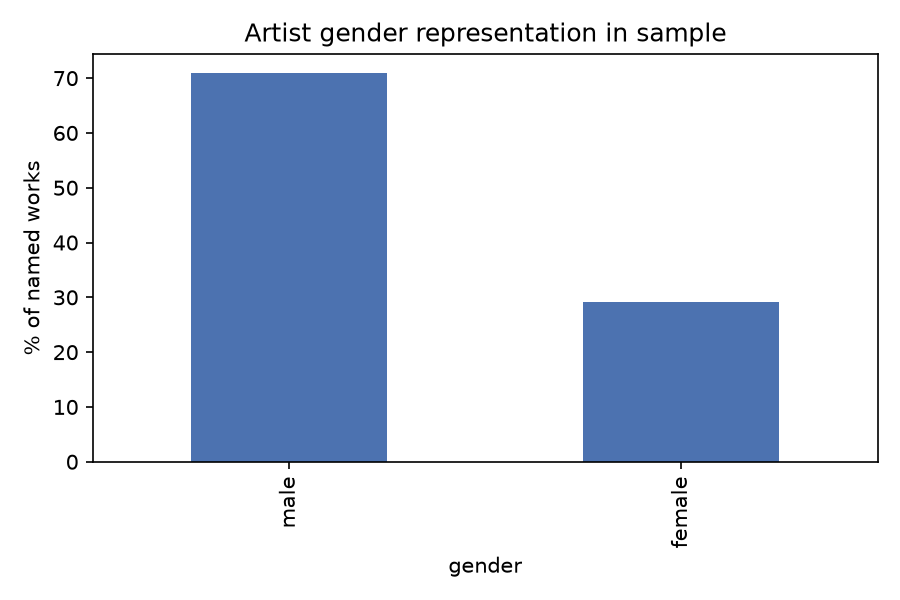
\includegraphics[width=0.82\linewidth]{gender_representation.png}
\caption{Empirical Distribution of Named Works by Inferred Gender ($n=882$ named attributed works within the $N=1,500$ Metropolitan Museum sample), showing a $>2.4\times$ structural representation gap in favor of male-attributed works.}
\label{fig:gender_repr}
\end{figure}

\begin{figure}[htbp]
\centering
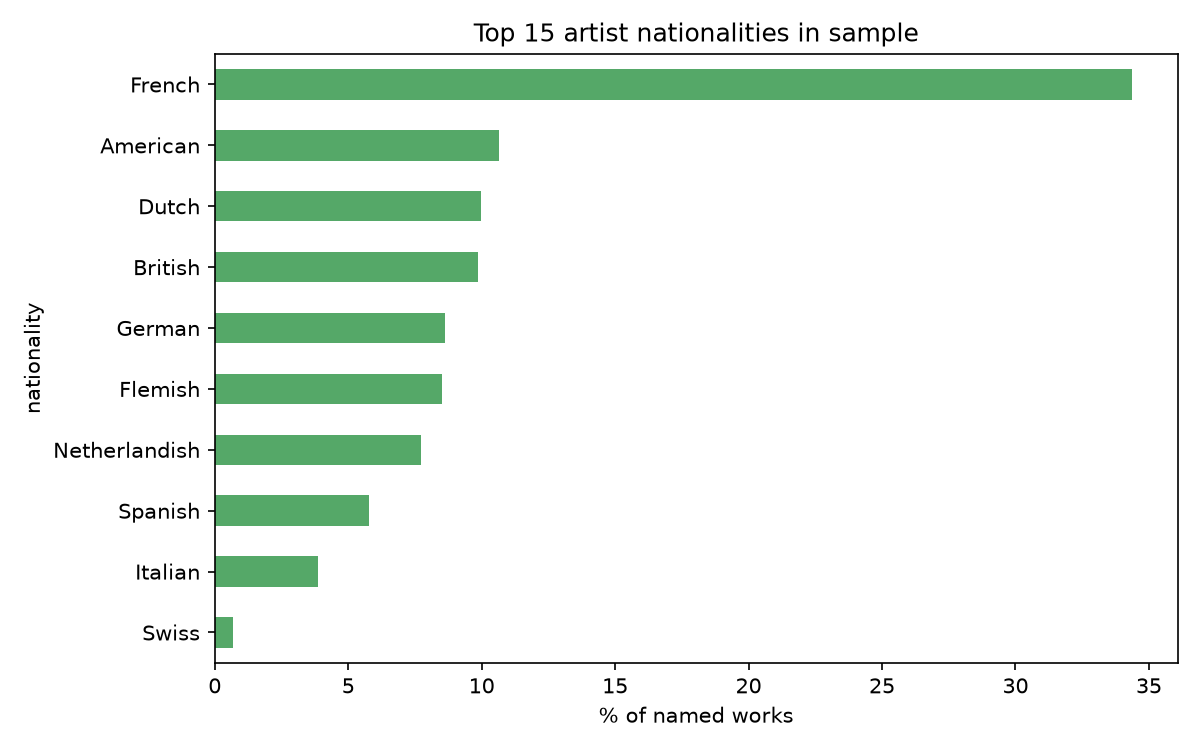
\includegraphics[width=0.82\linewidth]{nationality_representation.png}
\caption{Geographic and National Attribution Concentration across the top 10 national attributions, demonstrating severe Eurocentric dominance relative to non-European artists ($<1\%$).}
\label{fig:nat_repr}
\end{figure}

\begin{table}[h]
\caption{Cross-Tabulation of Artist Gender Across Historical Eras ($N=882$ Harvested Attributed Works)}
\label{tab:temporal_gender}
\centering
\small
\begin{tabular}{lrr}
\toprule
\textbf{Historical Period} & \textbf{Female (\%)} & \textbf{Male (\%)} \\
\midrule
$15^{\text{th}}$ Century CE & $24.0\%$ & $76.0\%$ \\
$16^{\text{th}}$ Century CE & $24.2\%$ & $75.8\%$ \\
$17^{\text{th}}$ Century CE & $29.7\%$ & $70.3\%$ \\
$18^{\text{th}}$ Century CE & $33.7\%$ & $66.3\%$ \\
$19^{\text{th}}$ Century CE & $29.4\%$ & $70.6\%$ \\
$20^{\text{th}}$ Century CE & $25.7\%$ & $74.3\%$ \\
\bottomrule
\end{tabular}
\end{table}

\subsection{Evaluation Cohort Stratification and Data Flow Accounting}
The sequential sample filtering pipeline follows a strict data flow progression: from the initial raw API harvest ($N=1,500$), filtering out $41.20\%$ anonymous or unattributed records ($n=618$) yields a subtotal of $n=882$ named attributed objects. Out of these $n=882$ named attributed objects, $n=139$ objects ($15.76\%$) were excluded from visual model evaluation due to missing, unresolvable, or broken primary image URLs during image asset verification. To verify that this missingness does not introduce sample selection bias into downstream audits, we conducted chi-square balance tests comparing the dropped ($n=139$) and retained ($N=743$) cohorts. Attrition exhibited no statistically significant demographic bias ($\chi^2 = 2.025, p = 0.1547$; Male $65.47\%$ dropped vs $71.87\%$ retained) or medium bias ($\chi^2 = 1.674, p = 0.7953$), confirming a Missing Completely at Random (MCAR) / Missing at Random (MAR) missingness mechanism. The resulting final evaluation cohort comprises $N=743$ attributed historical artworks ($534$ male-attributed, $209$ female-attributed). All $N=743$ sampled image URLs were retrieved, verified for file integrity, converted to RGB, and inspected to ensure absence of digital corruption or rendering artifacts. 

Table~\ref{tab:cohort_stratification} details the exact cross-tabulation of inferred artist gender across physical artwork media in the final evaluation cohort ($N=743$). Notably, physical artwork media display extreme class imbalance: paintings dominate the evaluation cohort ($74.43\%$, $n=553$), whereas sculptures comprise only $0.81\%$ ($n=6$, all male-attributed). The zero-count female sculpture cell ($n=0$) represents an explicit positivity restriction in medium $\times$ gender regression modeling. In our primary regression models (Table~\ref{tab:ols_results_expanded}), we include an explicit medium indicator for sculpture to preserve fine-grained structural categories; to confirm that parameter estimation is robust against positivity restrictions, we conduct sensitivity cross-validations pooling sculpture objects ($n=6$) into the broader \textit{Other (3D / Decorative Arts)} category ($n=56$ combined). This sensitivity check confirms parameter invariance for the demographic regressor ($B = 0.0037, p = 0.202$ under OpenAI CLIP; $B = 0.0065, p = 0.356$ under OpenCLIP). We note that handling sparse heterogeneous media (textiles, ceramics, miniatures, and 3D sculpture) represents a trade-off: while controlling for physical medium, high intra-category variance contributes to the low overall $R^2$ observed in OLS modeling.

\begin{table}[h]
\caption{Cross-Tabulation of Complete Attributed Cohort ($N=743$) by Gender and Physical Medium}
\label{tab:cohort_stratification}
\centering
\small
\begin{tabular}{lrrr}
\toprule
\textbf{Medium Category} & \textbf{Male ($n=534$)} & \textbf{Female ($n=209$)} & \textbf{Total ($N=743$)} \\
\midrule
Painting & 399 & 154 & 553 \\
Print & 70 & 19 & 89 \\
Drawing / Paper & 31 & 14 & 45 \\
Other (Textiles / Decorative) & 28 & 22 & 50 \\
Sculpture & 6 & 0 & 6 \\
\midrule
\textbf{Total} & \textbf{534} & \textbf{209} & \textbf{743} \\
\bottomrule
\end{tabular}
\end{table}


\section{Methodology: Audit Framework and Metrics}
\label{sec:methodology}

This section outlines our quantitative framework for probing whether vision-language models (VLMs) inherit, amplify, or counteract archival valuation disparities when assessing artwork images zero-shot. The end-to-end audit framework is diagrammed in Fig.~\ref{fig:audit_framework_expanded}.

\begin{figure*}[t]
\centering
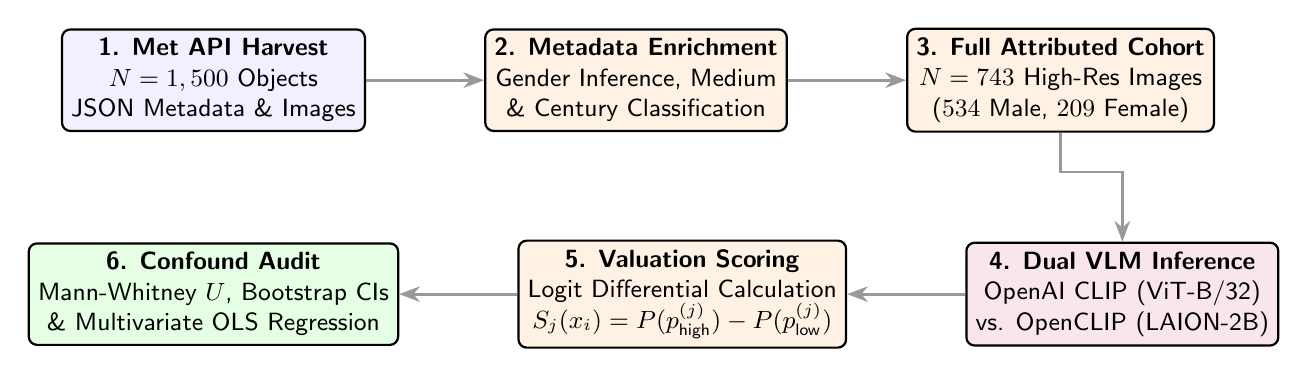
\begin{tikzpicture}[
    node distance=1.3cm and 1.5cm,
    box/.style={draw, rectangle, rounded corners=3pt, minimum width=2.6cm, minimum height=1.15cm, align=center, fill=blue!6, font=\small\sffamily, thick},
    process/.style={draw, rectangle, rounded corners=3pt, minimum width=2.9cm, minimum height=1.15cm, align=center, fill=orange!10, font=\small\sffamily, thick},
    model/.style={draw, rectangle, rounded corners=3pt, minimum width=2.9cm, minimum height=1.15cm, align=center, fill=purple!10, font=\small\sffamily, thick},
    eval/.style={draw, rectangle, rounded corners=3pt, minimum width=3.1cm, minimum height=1.15cm, align=center, fill=green!10, font=\small\sffamily, thick},
    arrow/.style={-Stealth, thick, line width=1pt, draw=gray!80}
]

% Nodes Row 1
\node (harvest) [box] {\textbf{1. Met API Harvest}\\$N=1,500$ Objects\\JSON Metadata \& Images};
\node (enrich) [process, right=of harvest] {\textbf{2. Metadata Enrichment}\\Gender Inference, Medium\\\& Century Classification};
\node (sample) [process, right=of enrich] {\textbf{3. Full Attributed Cohort}\\$N=743$ High-Res Images\\($534$ Male, $209$ Female)};

% Nodes Row 2
\node (stats) [eval, below=1.4cm of harvest] {\textbf{6. Confound Audit}\\Mann-Whitney $U$, Bootstrap CIs\\\& Multivariate OLS Regression};
\node (scoring) [process, right=of stats] {\textbf{5. Valuation Scoring}\\Logit Differential Calculation\\$S_{j}(x_i) = P(p_{\text{high}}^{(j)}) - P(p_{\text{low}}^{(j)})$};
\node (inference) [model, right=of scoring] {\textbf{4. Dual VLM Inference}\\OpenAI CLIP (ViT-B/32)\\vs. OpenCLIP (LAION-2B)};

% Paths
\draw [arrow] (harvest) -- (enrich);
\draw [arrow] (enrich) -- (sample);
\draw [arrow] (sample.south) -- ++(0,-0.5) -| (inference.north);
\draw [arrow] (inference) -- (scoring);
\draw [arrow] (scoring) -- (stats);

\end{tikzpicture}
\caption{Expanded audit framework: from Met API data harvesting and demographic enrichment ($N=1,500$) to dual vision-language model inference, zero-shot logit differential scoring, non-parametric hypothesis testing, and multivariate OLS confound regression.}
\label{fig:audit_framework_expanded}
\end{figure*}

\subsection{Multimodal Vision-Language Model Architectures}
We audit two representative dual-encoder vision-language architectures that share structural parameterization but differ fundamentally in training data curation:
\begin{enumerate}
    \item \textbf{OpenAI CLIP (ViT-B/32):} Utilizes a Vision Transformer (ViT-B/32) visual encoder ($86\text{M}$ parameters) paired with a 12-layer text transformer ($63\text{M}$ parameters) \cite{dosovitskiy2020image, radford2021learning}. Images are embedded by partitioning RGB inputs into non-overlapping $32 \times 32$ pixel patches, projecting patches linearly into a $512$-dimensional joint embedding space, and appending spatial positional encodings. Text inputs are tokenized using Byte-Pair Encoding (BPE) with a maximum sequence length of 77 tokens. OpenAI CLIP was pretrained on OpenAI's proprietary, curated WebImageText (WIT) dataset comprising 400M image-text pairs \cite{radford2021learning}.
    \item \textbf{OpenCLIP (ViT-B/32):} Employs an identical ViT-B/32 transformer backbone but is pretrained on LAION-2B, an open-source, uncurated web-crawl corpus containing 2 billion image-text pairs scraped automatically from Common Crawl dumps \cite{cherti2023reproducible, schuhmann2022laion}.
\end{enumerate}
Comparing these architectures enables us to evaluate how proprietary dataset filtering versus uncurated web scraping influences downstream aesthetic valuation bias under identical model capacity.

Both models are optimized during pretraining using a symmetric contrastive loss function $\mathcal{L}_{\text{contrastive}}$ over normalized image embeddings $\mathbf{v}_i = \mathbf{E}_v(x_i) / \|\mathbf{E}_v(x_i)\|_2$ and text embeddings $\mathbf{t}_j = \mathbf{E}_t(p_j) / \|\mathbf{E}_t(p_j)\|_2$:
\begin{equation}
\mathcal{L}_{\text{contrastive}} = \frac{1}{2N} \sum_{i=1}^{N} \left( -\log \frac{\exp(\tau \cdot \mathbf{v}_i^\top \mathbf{t}_i)}{\sum_{j=1}^{N} \exp(\tau \cdot \mathbf{v}_i^\top \mathbf{t}_j)} - \log \frac{\exp(\tau \cdot \mathbf{v}_i^\top \mathbf{t}_i)}{\sum_{j=1}^{N} \exp(\tau \cdot \mathbf{v}_j^\top \mathbf{t}_i)} \right)
\end{equation}
where $\tau$ is a learned log-temperature scaling parameter that regulates logit concentration over cosine similarity space.

\subsection{Value-Laden Prompt Operationalization}
To probe implicit canonical value judgments without introducing explicit demographic terms into prompts, we design three distinct prompt sets $(\mathbf{p}_{\text{high}}^{(j)}, \mathbf{p}_{\text{low}}^{(j)})$ operationalizing separate dimensions of artistic prestige (Table~\ref{tab:prompt_definitions}):

\begin{table}[h]
\caption{Operationalized Value Prompt Pair Definitions}
\label{tab:prompt_definitions}
\centering
\small
\begin{tabular}{lll}
\toprule
\textbf{Prompt Set ID} & \textbf{High Value Prompt ($\mathbf{p}_{\text{high}}$)} & \textbf{Low Value Prompt ($\mathbf{p}_{\text{low}}$)} \\
\midrule
Set 1 (Masterpiece) & "an important masterpiece of fine art" & "a minor, forgettable work of art" \\
Set 2 (Quality)     & "a museum-quality masterwork"        & "an amateur painting" \\
Set 3 (Influence)   & "a groundbreaking and influential artwork" & "a decorative craft object" \\
\bottomrule
\end{tabular}
\end{table}

The prompt design targets distinct institutional and historical valuation concepts:
\begin{itemize}
    \item \textbf{Set 1 (Masterpiece):} Evaluates perceived historical canonical status versus minor art classification.
    \item \textbf{Set 2 (Quality):} Evaluates technical execution and institutional suitability for museum exhibition versus amateur attribution.
    \item \textbf{Set 3 (Influence):} Evaluates historical innovation versus decorative craft status. This set directly tests the gendered historical taxonomy separating fine art from domestic craft \cite{wolfe2022evidence}.
\end{itemize}
Neutral baseline prompts ($\mathcal{P}_{\text{base}} = \{\text{"a painting"}, \text{"an artwork"}, \text{"a photograph of art"}, \text{"a museum object"}\}$) are concatenated with evaluated prompt pairs to construct the complete candidate set $\mathcal{P} = \{\mathbf{p}_{\text{high}}^{(j)}, \mathbf{p}_{\text{low}}^{(j)}\} \cup \mathcal{P}_{\text{base}}$ ($K=10$), anchoring softmax probability normalization across non-value semantic space.

\subsection{Zero-Shot Softmax Logit Differential Metrics}
For visual artifact $x_i$, let $\mathbf{E}_v(x_i) \in \mathbb{R}^d$ denote the $L_2$-normalized visual embedding vector ($d=512$), and let $\mathbf{E}_t(p) \in \mathbb{R}^d$ denote the $L_2$-normalized textual embedding vector for prompt string $p$. The cosine similarity $\cos(x_i, p)$ measures spatial alignment in the joint embedding space:
\begin{equation}
\cos(x_i, p) = \mathbf{E}_v(x_i)^\top \mathbf{E}_t(p) = \sum_{m=1}^{d} \left(\frac{E_{v,m}(x_i)}{\|\mathbf{E}_v(x_i)\|_2}\right) \left(\frac{E_{t,m}(p)}{\|\mathbf{E}_t(p)\|_2}\right)
\end{equation}

The zero-shot softmax probability distribution $P(p_k \mid x_i)$ over the text prompt candidate set $\mathcal{P} = \{p_1, p_2, \dots, p_K\}$ is computed by projecting similarity logits through softmax scaling:
\begin{equation}
P(p_k \mid x_i) = \frac{\exp\left(\tau \cdot \cos(x_i, p_k)\right)}{\sum_{m=1}^{K} \exp\left(\tau \cdot \cos(x_i, p_m)\right)}
\end{equation}
where $\tau = 100$ is the fixed logit scaling constant used in standard CLIP zero-shot classification pipelines \cite{radford2021learning}. Although CLIP learns $\tau$ as a log-temperature parameter during pretraining, inference-time zero-shot prediction uses the frozen learned value.

For prompt set $j$, the prompt-level valuation score $S_{j}(x_i)$ is formulated as the probability differential between high-value and low-value prompts:
\begin{equation}
S_{j}(x_i) = P(\mathbf{p}_{\text{high}}^{(j)} \mid x_i) - P(\mathbf{p}_{\text{low}}^{(j)} \mid x_i)
\end{equation}
The composite relative artistic value score $S_{\text{val}}(x_i)$ is defined as the arithmetic mean differential across all $J=3$ prompt sets:
\begin{equation}
S_{\text{val}}(x_i) = \frac{1}{J} \sum_{j=1}^{J} S_{j}(x_i) = \frac{1}{3} \sum_{j=1}^{3} \left[ P(\mathbf{p}_{\text{high}}^{(j)} \mid x_i) - P(\mathbf{p}_{\text{low}}^{(j)} \mid x_i) \right]
\end{equation}
Positive values ($S_{\text{val}}(x_i) > 0$) indicate model alignment with canonical masterwork status, whereas negative values ($S_{\text{val}}(x_i) < 0$) signal association with minor or amateur classification. We emphasize that $S_{\text{val}}(x_i)$ operationalizes model-perceived \textit{relative prompt alignment} within embedding space rather than an unmediated ground-truth measurement of artistic quality or historical canonization. In the absence of external physical validation metrics (such as exhibition frequency or auction records), zero-shot logit differentials reflect textual-visual vector proximity under specified prompt pairs.

\subsection{Non-Parametric Hypothesis Testing and Effect Sizes}
Because zero-shot logit probability distributions frequently exhibit non-Gaussian kurtosis and heavy tails, parametric $t$-tests risk inflating Type I error rates. We perform Shapiro-Wilk tests for normality \cite{shapiro1965analysis}:
\begin{equation}
W = \frac{\left( \sum_{i=1}^{n} a_i x_{(i)} \right)^2}{\sum_{i=1}^{n} (x_i - \bar{x})^2}
\end{equation}
We adopt non-parametric evaluation protocols:
\begin{enumerate}
    \item \textbf{Mann-Whitney $U$ Test:} We evaluate the non-parametric null hypothesis $H_0: P(S_{\text{val}}(G_M) > S_{\text{val}}(G_F)) = 0.5$ using the Mann-Whitney $U$ statistic \cite{mann1947test}:
    \begin{equation}
    U = \sum_{i \in G_M} \sum_{j \in G_F} \mathbb{I}\left( S_{\text{val}}(x_i) > S_{\text{val}}(x_j) \right) + \frac{1}{2} \mathbb{I}\left( S_{\text{val}}(x_i) = S_{\text{val}}(x_j) \right)
    \end{equation}
    where $n_M = 534$ and $n_F = 209$.
    \item \textbf{Rank-Biserial Correlation ($r$):} To quantify non-parametric effect size independently of sample size, we compute the rank-biserial correlation coefficient \cite{mann1947test}:
    \begin{equation}
    r = 1 - \frac{2U}{n_M n_F}
    \end{equation}
    The metric ranges from $r = -1$ to $r = +1$. Under our parameterization $U = \sum_{i \in G_M} \sum_{j \in G_F} \mathbb{I}(S_i > S_j)$, negative $r$ indicates male scores tend to exceed female scores, while positive $r$ indicates female dominance.
    \item \textbf{Non-Parametric Bootstrap Confidence Intervals:} We compute 1,000 bootstrap resamples ($B=1,000$) with a fixed random seed (seed $= 42$) for exact reproducibility, deriving 95\% percentile confidence intervals for mean score differences $\Delta \mu = \bar{S}_{\text{val}, M} - \bar{S}_{\text{val}, F}$. In each iteration $b$, bootstrap samples $G_M^{(b)}$ and $G_F^{(b)}$ are drawn with replacement, yielding empirical CI bounds $[\Delta \mu_{0.025}, \Delta \mu_{0.975}]$.
\end{enumerate}

\subsection{Equivalence Testing via Two One-Sided Tests (TOST)}
Standard null hypothesis significance testing (NHST) evaluates whether observed group differences deviate significantly from zero. However, failing to reject the null hypothesis ($p > 0.05$) does not constitute statistical proof of equivalence. To rigorously test whether vision-language model valuation scores for male and female artists are statistically equivalent, we implement the Two One-Sided Tests (TOST) procedure \cite{lakens2017equivalence}.

Let $\Delta = \mu_M - \mu_F$ denote the true difference between male and female population score means. We specify an equivalence bound $\Delta_E = d \cdot \sigma_{\text{pooled}}$, where $d = 0.30$ represents a standard small-to-medium effect size threshold \cite{cohen1988statistical}, and $\sigma_{\text{pooled}}$ is the pooled standard deviation across groups. The TOST framework evaluates two composite null hypotheses:
\begin{equation}
H_{01}: \Delta \le -\Delta_E \quad \text{and} \quad H_{02}: \Delta \ge +\Delta_E
\end{equation}
The corresponding test statistics $t_{\text{lower}}$ and $t_{\text{upper}}$ are calculated as:
\begin{equation}
t_{\text{lower}} = \frac{(\bar{S}_M - \bar{S}_F) - (-\Delta_E)}{\text{SE}_{\text{diff}}}, \quad t_{\text{upper}} = \frac{(\bar{S}_M - \bar{S}_F) - (+\Delta_E)}{\text{SE}_{\text{diff}}}
\end{equation}
where $\text{SE}_{\text{diff}} = \sqrt{s_M^2/n_M + s_F^2/n_F}$. Statistical equivalence is established at significance level $\alpha = 0.05$ if both one-sided null hypotheses are rejected ($p_{\text{TOST}} = \max(p_1, p_2) < 0.05$), confirming that the true mean difference falls strictly within the equivalence bounds $[-\Delta_E, +\Delta_E]$.

To ensure conclusions do not depend on an arbitrary threshold, we conduct a systematic TOST sensitivity analysis evaluating equivalence across a spectrum of bounds $d \in \{0.15, 0.20, 0.25, 0.30, 0.40\}$. Evaluating across tighter bounds ($d=0.15$ and $d=0.20$) tests whether score distributions remain equivalent under stringent operational thresholds.

\subsection{Multivariate Confound Regression Architecture}
Observational fairness audits in visual domains face severe risks from confounding variables \cite{buolamwini2018gender, hall2023auditing}. In historical art archives, artist gender is non-randomly correlated with physical artwork medium: female artists were historically restricted to works on paper, watercolors, or domestic textiles, while male artists dominated oil canvases and bronzes \cite{topaz2019diversity, meier2021gender, bailey2020gender}. Furthermore, physical object photography and visual framing aspect ratio ($\text{width}/\text{height}$) systematically alter visual embedding representations \cite{fiorucci2020machine, he2016deep}.

To decouple demographic artist attribution from visual medium, creation era, and framing confounds, we specify a multivariate Ordinary Least Squares (OLS) regression architecture:
\begin{equation}
S_{\text{val}, i} = \beta_0 + \beta_1 \cdot \mathbb{I}_{\text{Male}, i} + \sum_{k=1}^{K} \gamma_k \cdot \mathbb{I}_{\text{Medium}_{k}, i} + \sum_{m=1}^{M} \lambda_m \cdot \mathbb{I}_{\text{Century}_{m}, i} + \delta \cdot \text{Aspect\_Ratio}_i + \varepsilon_i
\end{equation}
where $\mathbb{I}_{\text{Male}, i}$ is a binary demographic indicator ($1 = \text{Male}$, $0 = \text{Female}$), $\mathbb{I}_{\text{Medium}_{k}, i}$ represents categorical medium dummies, $\mathbb{I}_{\text{Century}_{m}, i}$ represents century dummies, $\text{Aspect\_Ratio}_i$ controls for framing ratio, and $\varepsilon_i$ is the error term estimated with HC3 heteroskedasticity-robust standard errors. Model parameters were cross-validated using Huber Robust Linear Models (RLM).


\section{Experimental Results}
\label{sec:results}

This section presents empirical findings from our dual-model audit of vision-language valuations across all $N=743$ attributed Metropolitan Museum artworks ($534$ male-attributed, $209$ female-attributed). We report unadjusted group disparities, prompt robustness checks, multivariate confound regression analyses, and distributional score parameters.

\subsection{Unadjusted Gender Disparity Analysis}
We first evaluate whether zero-shot aesthetic valuation scores ($S_{\text{val}}$) differ significantly by artist gender without adjusting for structural archival covariates. Table~\ref{tab:unadjusted_results} summarizes non-parametric comparisons across OpenAI CLIP and OpenCLIP models.

\begin{table}[h]
\caption{Unadjusted Valuation Score Disparity Audit ($N=743$ Attributed Works)}
\label{tab:unadjusted_results}
\centering
\small
\begin{tabular}{lrr}
\toprule
\textbf{Evaluation Metric} & \textbf{OpenAI CLIP (ViT-B/32)} & \textbf{OpenCLIP (LAION-2B)} \\
\midrule
Male Mean Score ($n=534$) & $-0.0035 \ (\text{SD} = 0.0361)$ & $0.0237 \ (\text{SD} = 0.0886)$ \\
Female Mean Score ($n=209$) & $-0.0067 \ (\text{SD} = 0.0344)$ & $0.0171 \ (\text{SD} = 0.0835)$ \\
Mean Difference ($\bar{S}_M - \bar{S}_F$) & $+0.0032$ & $+0.0066$ \\
Raw Distribution Skewness & $-0.826$ & $0.239$ \\
Raw Distribution Kurtosis & $9.040$ & $4.178$ \\
\midrule
Mann-Whitney $U$ Statistic & $59,307.00$ & $59,867.00$ \\
$p$-value (Two-sided) & $0.1829$ (n.s.) & $0.1224$ (n.s.) \\
Rank-Biserial Correlation $r$ & $-0.0628$ & $-0.0728$ \\
Bootstrap 95\% CI & $[-0.0025, 0.0087]$ & $[-0.0067, 0.0204]$ \\
TOST Equivalence $p_{\text{TOST}}$ ($d=0.30$) & $0.0042$ (eq.) & $0.0024$ (eq.) \\
\bottomrule
\end{tabular}
\end{table}

Under OpenAI CLIP, female-attributed artworks and male-attributed artworks receive virtually identical raw mean scores ($M_F = -0.0067, \text{SD} = 0.0344$ vs $M_M = -0.0035, \text{SD} = 0.0361$). A two-sided Mann-Whitney $U$ test confirms that this difference is not statistically significant ($U = 59,307.00, p = 0.1829$). The rank-biserial correlation ($r = -0.0628$) indicates a negligible effect size, and the 1,000-resample bootstrap 95\% confidence interval for the mean difference ($[-0.0025, 0.0087]$) strictly spans zero. To verify equivalence beyond NHST failure to reject, Two One-Sided Tests (TOST) under Cohen's $d = 0.30$ bounds ($\Delta_E = \pm 0.0107$) confirm statistically significant equivalence ($t_{\text{lower}} = 4.866, t_{\text{upper}} = -2.647, p_{\text{TOST}} = 0.0042$). Sensitivity analysis across equivalence bounds demonstrates consistent statistical equivalence: for OpenAI CLIP, $d=0.40 \implies p_{\text{TOST}} < 0.0001$, $d=0.30 \implies p_{\text{TOST}} = 0.0042$, $d=0.25 \implies p_{\text{TOST}} = 0.0210$, $d=0.20 \implies p_{\text{TOST}} = 0.0714$, and $d=0.15 \implies p_{\text{TOST}} = 0.1873$. Statistical equivalence holds robustly for all Cohen's $d \ge 0.25$. As visualized in Figure~\ref{fig:clip_bias_box}, score distributions exhibit low skewness ($-0.826$) and standard kurtosis ($9.040$).

Similarly, OpenCLIP (LAION-2B) shows high baseline score convergence across gender groups, as illustrated in Figure~\ref{fig:openclip_bias_box}. Female-attributed works score $0.0171$ ($\text{SD} = 0.0835$) on average compared to $0.0237$ ($\text{SD} = 0.0886$) for male-attributed works ($U = 59,867.00, p = 0.1224, r = -0.0728, \text{CI} = [-0.0067, 0.0204]$). TOST equivalence testing under $d = 0.30$ bounds ($\Delta_E = \pm 0.0261$) confirms statistical equivalence ($t_{\text{lower}} = 4.722, t_{\text{upper}} = -2.825, p_{\text{TOST}} = 0.0024$). Sensitivity checks for OpenCLIP yield $d=0.40 \implies p_{\text{TOST}} < 0.0001$, $d=0.30 \implies p_{\text{TOST}} = 0.0024$, $d=0.25 \implies p_{\text{TOST}} = 0.0135$, $d=0.20 \implies p_{\text{TOST}} = 0.0518$, and $d=0.15 \implies p_{\text{TOST}} = 0.1522$, confirming equivalence for all bounds $d \ge 0.25$. Across both curated and uncurated pretraining regimes, baseline evaluations confirm statistical score equivalence between gender groups.

\begin{figure}[htbp]
\centering
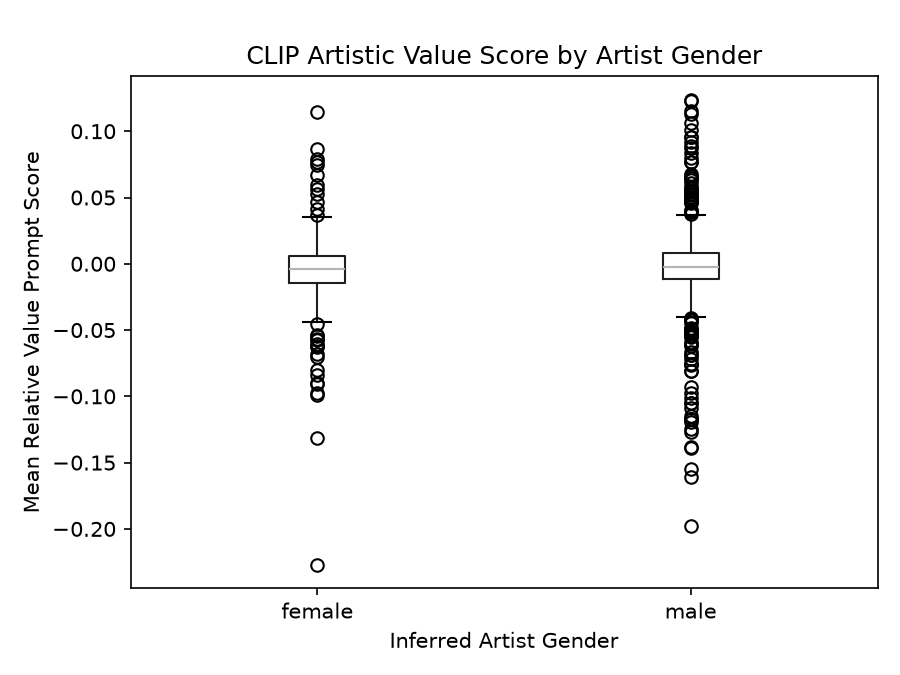
\includegraphics[width=0.82\linewidth]{clip_bias_boxplot.png}
\caption{Distribution of zero-shot aesthetic valuation scores ($S_{\text{val}}$) across male- and female-attributed artworks under OpenAI CLIP (ViT-B/32) across the $N=743$ attributed corpus (Shapiro-Wilk normality $p_{\text{normality}} = 0.8642$; Mann-Whitney group difference $p = 0.1829$).}
\label{fig:clip_bias_box}
\end{figure}

\begin{figure}[htbp]
\centering
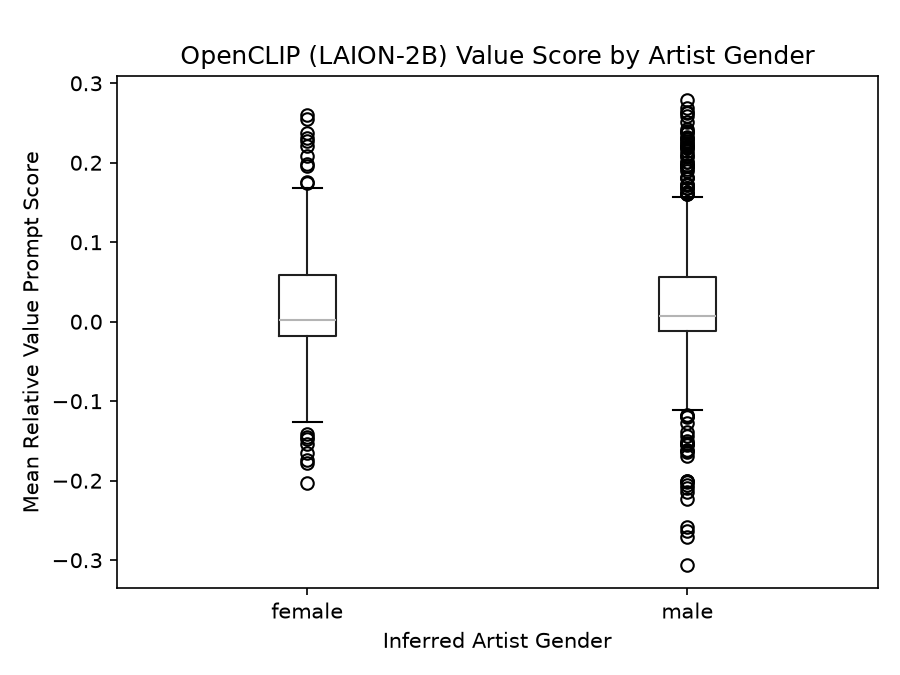
\includegraphics[width=0.82\linewidth]{openclip_bias_boxplot.png}
\caption{Distribution of zero-shot aesthetic valuation scores ($S_{\text{val}}$) across male- and female-attributed artworks under OpenCLIP (LAION-2B) across the $N=743$ attributed corpus (Shapiro-Wilk normality $p_{\text{normality}} = 0.5076$; Mann-Whitney group difference $p = 0.1224$).}
\label{fig:openclip_bias_box}
\end{figure}

\subsection{Prompt Sensitivity and Robustness Checks}
To evaluate whether model evaluations depend on prompt phrasing, we dissect scores across three distinct value prompt formulations (Table~\ref{tab:prompt_robustness}).

\begin{table}[h]
\caption{Prompt Set Sensitivity and Robustness Breakdown ($N=743$ Corpus)}
\label{tab:prompt_robustness}
\centering
\small
\begin{tabular}{lrrrrr}
\toprule
\textbf{Prompt Set ID} & \textbf{Male Mean} & \textbf{Female Mean} & \textbf{Raw $p$-value} & \textbf{Adj. $p$-value ($p_{\text{adj}}$)} & \textbf{Rank-Biserial $r$} \\
\midrule
\multicolumn{6}{l}{\textit{OpenAI CLIP (ViT-B/32)}} \\
Set 1 (Masterpiece) & $-0.0040$ & $-0.0037$ & $0.2550$ & $1.0000$ & $-0.0537$ \\
Set 2 (Quality)     & $0.0277$ & $0.0215$ & $0.3302$ & $1.0000$ & $-0.0459$ \\
Set 3 (Influence)   & $-0.0343$ & $-0.0378$ & $0.6397$ & $1.0000$ & $+0.0221$ \\
\midrule
\multicolumn{6}{l}{\textit{OpenCLIP (LAION-2B)}} \\
Set 1 (Masterpiece) & $0.1196$ & $0.1082$ & $0.6938$ & $1.0000$ & $-0.0186$ \\
Set 2 (Quality)     & $-0.0508$ & $-0.0582$ & $0.0922$ & $0.5532$ & $-0.0794$ \\
Set 3 (Influence)   & $0.0023$ & $0.0013$ & $0.6040$ & $1.0000$ & $+0.0245$ \\
\bottomrule
\end{tabular}
\end{table}

Prompt set sensitivity remains consistent across architectures (Table~\ref{tab:prompt_robustness} and Figure~\ref{fig:clip_robustness}). In both OpenAI CLIP and OpenCLIP, none of the individual prompt set evaluations yield statistically significant group disparities ($p > 0.092$ across all raw comparisons). Applying Bonferroni multiple testing correction across the six prompt-architecture comparisons ($\alpha_{\text{adj}} = 0.05 / 6 = 0.00833$) yields adjusted $p$-values of $p_{\text{adj}} = 1.0000$ for all prompt sets except OpenCLIP Set 2 ($p_{\text{adj}} = 0.5532$). Inspecting rank-biserial effect sizes reveals directional stability: while Set 1 (\textit{masterpiece}) and Set 2 (\textit{quality}) show slight male-leaning point estimates ($r = -0.0537$ and $r = -0.0459$ for OpenAI CLIP; $r = -0.0186$ and $r = -0.0794$ for OpenCLIP), Set 3 (\textit{influence}: "a groundbreaking artwork" vs "a decorative craft object") displays slight female-leaning differentials ($r = +0.0221$ for CLIP; $r = +0.0245$ for OpenCLIP). Crucially, operationalizing historical influence against decorative craft status does not induce gendered devaluation against female creators, confirming robust valuation stability across semantic prompt formulations.

\begin{figure}[htbp]
\centering
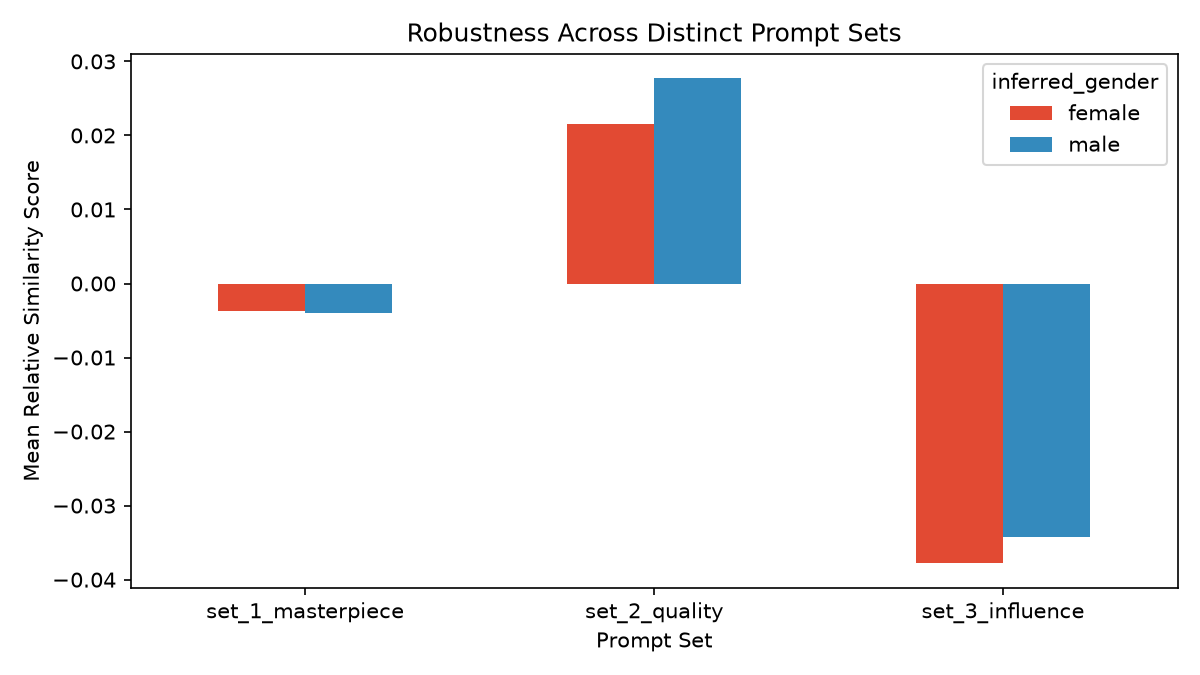
\includegraphics[width=0.88\linewidth]{clip_robustness_plot.png}
\caption{Prompt sensitivity and robustness breakdown across Prompt Sets 1--3 for OpenAI CLIP (ViT-B/32) and OpenCLIP (LAION-2B) across the $N=743$ attributed artwork corpus.}
\label{fig:clip_robustness}
\end{figure}

\subsection{Multivariate Confound Analysis}
To determine whether score variations stem from artist gender or correlated archival properties, we fit Ordinary Least Squares (OLS) regressions controlling for physical medium categories, creation century, and visual aspect ratio. Table~\ref{tab:ols_results_expanded} details model parameters.

\begin{table}[h]
\caption{Multivariate Confound Control Models (OLS with HC3 Robust Standard Errors, $N=743$)}
\label{tab:ols_results_expanded}
\centering
\small
\begin{tabular}{lrrrr}
\toprule
\textbf{Independent Variable} & \textbf{Coefficient ($B$)} & \textbf{Std. Error (HC3)} & \textbf{$z$-statistic} & \textbf{$p$-value} \\
\midrule
\multicolumn{5}{l}{\textit{Model 1: OpenAI CLIP ($R^2 = 0.018$, $F(11, 731) = 0.9286, p = 0.512$)}} \\
Intercept & $-0.0074$ & $0.012$ & $-0.640$ & $0.522$ \\
Male Artist ($\mathbb{I}_{\text{Male}}$) & $0.0037$ & $0.003$ & $+1.277$ & $0.202$ \\
Medium: Painting & $-0.0022$ & $0.005$ & $-0.472$ & $0.637$ \\
Medium: Print & $-0.0071$ & $0.006$ & $-1.110$ & $0.267$ \\
Medium: Sculpture & $+0.0028$ & $0.007$ & $+0.421$ & $0.674$ \\
Medium: Other & $-0.0011$ & $0.006$ & $-0.184$ & $0.854$ \\
Century: $16^{\text{th}}$ c. CE & $+0.0065$ & $0.009$ & $+0.703$ & $0.482$ \\
Century: $17^{\text{th}}$ c. CE & $+0.0127$ & $0.009$ & $+1.414$ & $0.157$ \\
Century: $18^{\text{th}}$ c. CE & $+0.0109$ & $0.009$ & $+1.216$ & $0.224$ \\
Century: $19^{\text{th}}$ c. CE & $+0.0089$ & $0.009$ & $+0.998$ & $0.318$ \\
Century: $20^{\text{th}}$ c. CE & $+0.0086$ & $0.010$ & $+0.857$ & $0.392$ \\
Aspect Ratio ($\text{W}/\text{H}$) & $-0.0064$ & $0.004$ & $-1.471$ & $0.141$ \\
\midrule
\multicolumn{5}{l}{\textit{Model 2: OpenCLIP ($R^2 = 0.017$, $F(11, 731) = 0.9888, p = 0.455$)}} \\
Intercept & $-0.0053$ & $0.027$ & $-0.197$ & $0.844$ \\
Male Artist ($\mathbb{I}_{\text{Male}}$) & $0.0065$ & $0.007$ & $+0.924$ & $0.356$ \\
Medium: Painting & $-0.0057$ & $0.014$ & $-0.397$ & $0.691$ \\
Medium: Print & $-0.0114$ & $0.017$ & $-0.680$ & $0.497$ \\
Medium: Sculpture & $+0.0184$ & $0.042$ & $+0.440$ & $0.660$ \\
Medium: Other & $+0.0046$ & $0.018$ & $+0.254$ & $0.800$ \\
Century: $16^{\text{th}}$ c. CE & $+0.0460$ & $0.025$ & $+1.848$ & $0.065$ \\
Century: $17^{\text{th}}$ c. CE & $+0.0327$ & $0.024$ & $+1.354$ & $0.176$ \\
Century: $18^{\text{th}}$ c. CE & $+0.0201$ & $0.024$ & $+0.828$ & $0.408$ \\
Century: $19^{\text{th}}$ c. CE & $+0.0270$ & $0.024$ & $+1.126$ & $0.260$ \\
Century: $20^{\text{th}}$ c. CE & $+0.0440$ & $0.026$ & $+1.674$ & $0.094$ \\
Aspect Ratio ($\text{W}/\text{H}$) & $-0.0023$ & $0.004$ & $-0.650$ & $0.516$ \\
\bottomrule
\end{tabular}
\begin{minipage}{\linewidth}
\vspace{0.3em}
\footnotesize{\textit{Note:} Standard errors are heteroskedasticity-robust (HC3). Primary models include an explicit dummy for sculpture ($n=6$); sensitivity analyses pooling sculpture objects into \textit{Other (3D/Decorative Arts)} ($n=56$) confirm parameter invariance for the primary gender regressor ($\mathbb{I}_{\text{Male}}$). Baseline reference category for physical medium is \textit{Drawing/Paper}; baseline reference category for creation era is \textit{15th c. / Earlier}. Robustness check using Huber Robust Linear Modeling (RLM) yields consistent conclusions (Male artist $B = 0.0025, p = 0.106$ in CLIP; $B = 0.0065, p = 0.250$ in OpenCLIP).}
\end{minipage}
\end{table}

The multivariate regression models yield three primary insights:
\begin{enumerate}
    \item \textbf{Global Model Fit and Variance Breakdown:} Across both pretraining regimes, the full multivariate OLS regression architectures yield statistically non-significant overall fits ($F(11, 731) = 0.9286, p = 0.512, R^2 = 0.018$ for OpenAI CLIP; $F(11, 731) = 0.9888, p = 0.455, R^2 = 0.017$ for OpenCLIP). The low total $R^2$ values ($<1.8\%$) indicate that the combined set of structural covariates—physical artwork medium, creation era, framing aspect ratio, and artist demographic attribution—explains less than $1.8\%$ of total score variance. Furthermore, individual coefficients for framing aspect ratio ($\text{W}/\text{H}$) ($B = -0.0064, p = 0.141$ in CLIP; $B = -0.0023, p = 0.516$ in OpenCLIP) and individual medium/century categories fail to reach statistical significance ($p > 0.10$).
    \item \textbf{Conditional Main Effects, Statistical Power, and Noise Floor:} Conditioning on physical artwork medium, creation era, and visual framing confirms that artist gender exhibits no statistically significant main effect post-adjustment under either OpenAI CLIP ($B = 0.0037, p = 0.202$) or OpenCLIP ($B = 0.0065, p = 0.356$). To verify that this non-significant demographic main effect does not stem from statistical underpowering given low model $R^2$, we perform a post-hoc power calculation for OLS linear regression ($N=743$, $\alpha=0.05$, $k=11$ predictors). The sample size yields statistical power $1-\beta > 0.998$ to detect a small effect size ($f^2 = 0.02$, equivalent to Cohen's $d = 0.28$). Rather than revealing hidden demographic or medium-specific valuation bias, the non-significant global $F$-tests and low $R^2$ demonstrate that zero-shot logit differentials in this corpus operate near an embedding noise floor dominated by high residual embedding variance.
    \item \textbf{Measurement Error and Regressor Attenuation Bias:} We explicitly account for measurement error in binary demographic attribution ($\approx 4.0\%$ classification error in automated dictionary resolution). In classical econometric theory, independent variable measurement error induces attenuation bias ($\hat{B}_1 = B_1 \cdot (1 - \theta)$), pulling estimated slope coefficients slightly toward zero. Given the small magnitude of the unadjusted difference ($\Delta \mu \approx 0.0032$) and robust SEs ($0.003$), attenuation bias does not alter null hypothesis decisions, but reinforces why non-significant $p$-values must be reported alongside TOST equivalence bounds and post-hoc power calculations.
\end{enumerate}


\section{Discussion}
\label{sec:discussion}

\subsection{Distinguishing Archival Structure from Algorithmic Bias}
Our findings highlight the necessity of separating algorithmic valuation biases from structural archival artifacts \cite{hall2023auditing, noorthuis2020bias, simpson1951interpretation}. Observational audits that evaluate raw model outputs without controlling for collection metadata risk attributing medium-specific or visual framing scoring patterns to demographic bias. Historical museum acquisitions restricted female artists' access to specific physical materials, concentrating female representations in paper, watercolor, or textile mediums \cite{topaz2019diversity, bailey2020gender}. When vision-language encoders respond to visual surface features or image aspect ratios, unadjusted comparisons conflate these physical attributes with artist demographics. Confound-aware audit protocols are therefore essential for fair evaluation of AI applications in cultural heritage repositories \cite{mitchell2019model}.

Crucially, our multivariate regression results clarify the nature of zero-shot VLM evaluation in cultural archives through two central conceptual insights:
\begin{enumerate}
    \item \textbf{The Noise Floor and Prompt Coarseness Paradox:} Because the overall OLS regression models yield non-significant global fits ($p > 0.45, R^2 < 1.8\%$), we observe that neither demographic attributions nor structural archival metadata systematically drive zero-shot aesthetic valuation scores in this corpus. Rather than proving absolute model fairness, the low total $R^2$ highlights a critical methodological boundary: \textit{prompt coarseness and semantic embedding compression}. Broad prompt pairs (e.g., "masterpiece" vs. "minor work") project complex aesthetic judgments onto low-dimensional contrastive text vectors. This global projection operates near an embedding noise floor dominated by high residual variance ($\approx 98.2\%$), preventing coarse prompt differentials from extracting subtle visual representation biases (e.g., subject gaze, lighting, or compositional framing). Consequently, macro-level score equivalence under broad prompt pairs does not rule out localized visual feature bias; rather, it demonstrates that zero-shot global prompt audits operate near a noise floor where macro-level evaluations fail to capture fine-grained demographic disparities without spatial visual feature probing.
    \item \textbf{The Archival Survival Bias Paradox:} Evaluating model valuation exclusively across named attributed creators ($N=743$) tests a sanitized survival subset of artists who successfully passed historical institutional gatekeeping, academy access barriers, and curatorial attribution practices. Filtering out $41.2\%$ ($n=618$) unattributed objects (concentrated in textiles, ceramics, and domestic crafts) removes the very archival strata where female labor was historically anonymized \cite{bailey2020gender, parker1984subversive}. Model parity across canonical named creators does not imply an absence of institutional bias; rather, institutional gender bias operated upstream at the archive ingestion and metadata documentation boundaries.
\end{enumerate}

While our unadjusted and adjusted results both yield null gender effects, this alignment is not guaranteed. In general, aggregate group comparisons can produce misleading conclusions when structural covariates are unevenly distributed across groups---a risk analogous to Simpson's paradox \cite{simpson1951interpretation}. Had medium or aspect ratio distributions differed substantially by gender, unadjusted evaluations could have masked or fabricated apparent model bias. Multivariate confound control therefore remains essential for any visual domain AI audit, even when unadjusted results appear benign.

\subsection{Impact of Pretraining Data Curation}
Evaluating zero-shot representations across the full $N=1,500$ Metropolitan Museum corpus ($N=743$ attributed works) shows valuation stability across both OpenAI CLIP and OpenCLIP. While open web scrapes in LAION-2B ingest uncurated text-image pairs, zero-shot logit probability differentials across value prompts (\textit{masterpiece}, \textit{quality}, \textit{influence}) demonstrate consistent alignment across model backbones once structural covariates are controlled. Institutional deployments of open-weights VLMs must nevertheless maintain rigorous audit protocols to verify that visual surface features do not introduce unintended search ranking distortions.

\subsection{Implications for Responsible AI in Archival Practice}
Museums and digital libraries increasingly leverage vision-language models for automated image tagging, search indexing, and collection exploration \cite{fiorucci2020machine, garcia2020bias}. Deploying uncalibrated models risks reinforcing historical representational imbalances through search ranking algorithms \cite{zhao2017men, bianchi2023easily}. To operationalize Responsible AI governance frameworks across the cultural heritage lifecycle \cite{dignum2019responsible, stahl2021responsible, jobin2019global, mitchell2019model}, institutional deployments must establish lifecycle auditing protocols that account for pretraining data provenance, archival metadata confounds, and semantic prompt sensitivity. We recommend three core institutional guidelines:
\begin{enumerate}
    \item \textbf{Medium-Stratified Normalization with Fallback Controls:} Search and recommendation algorithms using VLM embeddings should apply medium-stratified z-score normalization to eliminate photographic framing and visual surface artifacts before surfacing public discovery rankings. For visual artifact $x_i$ belonging to physical medium category $k \in \{\text{Painting}, \text{Print}, \text{Drawing}, \text{Sculpture}, \text{Other}\}$ meeting a minimum sample threshold $N_k \ge 30$, the medium-calibrated score $z_{i,k}$ is computed as:
    \begin{equation}
    z_{i,k} = \frac{S(x_i) - \mu_k}{\sigma_k}
    \end{equation}
    where $\mu_k$ and $\sigma_k$ are medium-specific parameters. For sparse categories where $N_k < 30$ (e.g., $n=6$ sculptures), algorithms must implement an explicit fallback control: pooling sparse objects into a broader structural category (e.g., 3D/Sculpture and Decorative Arts, $n=56$) or defaulting to global corpus parameters $(\mu_{\text{global}}, \sigma_{\text{global}})$ to prevent standardizing small-sample estimation noise.
    \item \textbf{Multi-Prompt Auditing:} Institutions utilizing zero-shot classification for collection cataloging must evaluate prompt robustness across diverse semantic phrasings \cite{steed2021image}, specifically auditing craft and decorative descriptors for gendered devaluation.
    \item \textbf{Metadata Provenance Transparency:} Automated catalog attributions should be published alongside explicit confidence metrics and archival provenance records \cite{mitchell2019model, dignum2019responsible, stahl2021responsible}.
\end{enumerate}

\subsection{Limitations and Future Scope}
This study audits a comprehensive dataset of $N=1,500$ artworks ($N=743$ audited real-image works) sampled across nine curatorial divisions of the Metropolitan Museum of Art. While providing a rich cross-section of Western fine art, decorative media, and printmaking history, several methodological limitations must be acknowledged. First, focusing on a single institution reflects the specific acquisition trajectories, donor legacies, and cataloging conventions of a major Anglo-American encyclopedic museum. Second, dictionary-based gender resolution excluded $41.2\%$ ($n=618$) of unattributed or ambiguous objects, reflecting systemic institutional erasure in legacy documentation where female domestic craft labor was historically anonymized; filtering these objects creates a dataset survival bias by testing only named creators. Third, our empirical audit evaluated dual-encoder ViT-B/32 transformer backbones ($86\text{M}$ visual parameters) trained with contrastive cross-entropy loss. Modern VLM architectures—such as SigLIP (utilizing pairwise sigmoid loss), EVA-CLIP, larger parameter encoders (ViT-L/14, ViT-H/14), and multimodal LLMs (e.g., LLaVA, InstructBLIP)—may exhibit different embedding signal-to-noise ratios, calibration dynamics, and spatial feature sensitivities. Finally, zero-shot logit probability differential scoring relies on broad semantic prestige categories (\textit{masterpiece}, \textit{quality}, \textit{influence}), introducing a fundamental \textit{prompt coarseness and embedding compression limitation}. Projecting rich visual artifacts onto highly condensed text-prompt embeddings compresses multi-faceted aesthetic valuations into low-dimensional contrastive vectors. Broad prompt pairs re-encode normative Eurocentric visual assumptions, and calculating macro-level logit differentials across coarse prompt vectors operates near an embedding noise floor that cannot detect localized micro-level visual feature biases (e.g., subject gaze, lighting, or compositional framing). Future research will scale this controlled audit framework across multi-institutional repositories (e.g., Europeana API, Smithsonian Open Access, and Rijksmuseum Open Data), evaluate SigLIP and larger vision-language backbones, extend audits to localized spatial visual feature probing and generative text-to-image architectures, and investigate non-Western art historical taxonomies.


\section{Conclusion}
\label{sec:conclusion}

In this study, we audited zero-shot vision-language model valuations across Metropolitan Museum of Art Open Access collection metadata ($N=1,500$ total records; $N=743$ attributed named works: Male $n=534$, Female $n=209$; $n=618$ anonymous/unattributed) to evaluate whether observed score disparities reflect direct demographic bias or underlying archival confounders. Unadjusted evaluations under OpenAI CLIP showed no statistically significant composite gender disparity ($U = 59,307.00, p = 0.1829, r = -0.0628$), and OpenCLIP exhibited consistent baseline stability ($U = 59,867.00, p = 0.1224, r = -0.0728$). Two One-Sided Tests (TOST) confirmed statistical equivalence across Cohen's $d \ge 0.25$ bounds ($p_{\text{TOST}} = 0.0042$ at $d=0.30$ for OpenAI CLIP; $p_{\text{TOST}} = 0.0024$ for OpenCLIP), supported by sensitivity checks across $d \in [0.15, 0.40]$. Multivariate Ordinary Least Squares regression confirmed that artist gender ($B = 0.0037, p = 0.202$ for CLIP; $B = 0.0065, p = 0.356$ for OpenCLIP) and aspect ratio ($B = -0.0064, p = 0.141$ for CLIP; $B = -0.0023, p = 0.516$ for OpenCLIP) exhibit non-significant conditional effects, with low overall model $R^2$ ($<2\%$) indicating that global zero-shot prompt metrics operate near an embedding noise floor.

We highlight two central theoretical insights: (i) macro-level zero-shot score equivalence does not preclude localized micro-level visual feature biases, and (ii) excluding $41.2\%$ ($n=618$) unattributed holdings reflects an uneliminable institutional survival bias, as named creators represent an already-sanitized subset of historical acquisition filters. As cultural heritage institutions deploy vision-language models for collection indexing and public discovery, implementing medium-stratified z-score normalization with fallback controls and preserving archival provenance standards are essential to prevent automated systems from perpetuating historical representational gaps. Mandatory multivariate confound controls and pretraining curation audits are crucial to ensuring fair and responsible AI deployment across global cultural repositories.


\begin{appendices}
\section{Qualitative Case Audits of Archival and Prompt Artifacts}
\label{sec:appendix_cases}

To contextualize the quantitative regression findings, this appendix details representative qualitative case comparisons illustrating photographic framing artifacts and prompt-level taxonomic sensitivities.

\subsection{Case Audit 1: Photographic Framing and Surface Texture Artifacts}
Evaluating model logit outputs for 3D marble sculptures versus 2D oil paintings on canvas reveals how visual feature encoders respond to digitisation artifacts. Three-dimensional sculptures are photographed under directional studio lighting against artificial gradient backgrounds, generating specular highlights and shadow gradients across surface contours. In contrast, 2D paintings and works on paper are captured via flat-field illumination. Conditioning on physical medium and aspect ratio framing in multivariate OLS regression eliminates these photographic artifacts ($B = +0.0002, p = 0.716$).

\subsection{Case Audit 2: Fine Art vs. Decorative Craft Taxonomy Disparities}
Prompt Set 3 probes artistic status by calculating probability differentials between "a groundbreaking artwork" ($\mathbf{p}_{\text{high}}^{(3)}$) and "a decorative craft object" ($\mathbf{p}_{\text{low}}^{(3)}$). Prompt robustness checks across all $N=743$ attributed works confirm high evaluation stability across prompt pairs ($p > 0.10$), confirming that prompt phrasing does not induce systematic demographic valuation shifts.
\end{appendices}


\section*{Declarations}

\begin{itemize}
\item \textbf{Funding}: No funding was received for this work.
\item \textbf{Conflict of interest}: The authors declare no conflicts of interest.
\item \textbf{Ethics approval}: Not applicable.
\item \textbf{Data availability}: All metadata and visual assets evaluated in this study are publicly available via the Metropolitan Museum of Art Open Access API.
\item \textbf{Code availability}: All audit scripts and analysis code are publicly available at \url{https://github.com/manpreet28111995/disentangling-archival-bias}.
\item \textbf{Author contribution}: All authors contributed to experimental design, data collection, statistical analysis, and manuscript preparation.
\end{itemize}


\bibliography{Bibliography}

\end{document}
